\documentclass[10pt,a4paper,twocolumn]{article}
\usepackage[utf8]{inputenc}
\usepackage[T1]{fontenc}
\usepackage[margin=1.6cm,top=1.8cm,bottom=1.8cm,columnsep=0.65cm]{geometry}
\usepackage{graphicx}
\usepackage{booktabs}
\usepackage{amsmath,amssymb}
\usepackage{array}
\usepackage{caption}
\usepackage{xcolor}
\usepackage{hyperref}
\usepackage{float}

\renewcommand{\figurename}{Figura}
\renewcommand{\tablename}{Tabela}
\renewcommand{\refname}{Refer\^encias Bibliogr\'aficas}
\renewcommand{\abstractname}{Resumo Executivo}

\captionsetup{font=small,labelfont=bf,skip=4pt}
\definecolor{darkblue}{RGB}{20,50,110}
\hypersetup{
    colorlinks=true,
    linkcolor=darkblue,
    citecolor=darkblue,
    urlcolor=darkblue
}

\setlength{\parskip}{3pt}
\setlength{\parindent}{1em}

\title{\vspace{-0.8cm}\textbf{\Large Genômica Comparada da Longevidade, Encefalização e Resistência ao Câncer em Psittaciformes: Remodelagem Telomérica em Linhagens de Vida Curta e Coevolução Proteômica entre Cérebro e Longevidade}}

\author{
\textbf{Angelo}\\
\small Centro Universitário do Planalto Central Apparecido dos Santos (UNICEPLAC), Brasília, DF, Brasil\\
\small Repositório reprodutível: \texttt{github.com/redkk123/Parrots} (\texttt{claude/new-session-lwh7xh})
}

\date{\small 10 de novembro de 2026 — Relatório Científico Consolidado (Mini-Paper)}

\begin{document}

\twocolumn[{
  \begin{@twocolumnfalse}
    \maketitle
    \vspace{-0.4cm}
    \begin{abstract}
    \noindent \textbf{Resumo.} Os psitacídeos (ordem Psittaciformes) combinam longevidade extrema (50--80 anos em araras, cacatuas, amazonas e no kakapo \textit{Strigops habroptila}) e encefalização comparável à de primatas com linhagens de vida curta e alta incidência tumoral, notadamente o periquito-australiano (\textit{Melopsittacus undulatus}). Neste estudo pré-registrado, integramos epidemiologia comparada de neoplasias (15.881 necropsias em duas bases independentes), alometria filogenética em duas topologias (supertree de Burgio et al.\ 2019 e árvore molecular de Smith et al.\ 2024), auditoria de qualidade e identidade de 126 montagens genômicas (\texttt{compleasm}/\texttt{aves\_odb10} e distâncias nucleares Mash), testes de seleção molecular (HyPhy RELAX e aBSREL) num painel de 101 genes (módulos M1--M8) confrontado com um modelo nulo de 298 genes e verificação em reads brutos do SRA, e correlações genômicas de taxa evolutiva relativa (\texttt{RERconverge}) em 7.756 genes codificantes (1.000 permulações filogenéticas) em 58 espécies. Primeiro, demonstramos que \textit{M.\ undulatus} é um \textit{outlier} verdadeiro de neoplasia (20,8--23,2\% vs.\ 1,5--5,0\% em lóris, $p \le 10^{-16}$), enquanto a suposta redução de longevidade na família Psittaculidae inteira é sensível à árvore ($p = 0,003$ em Burgio vs.\ $p = 0,050$ em Smith). Segundo, nossa auditoria de 126 genomas revelou contaminação mitocondrial cruzada em 62/96 montagens \textit{short-read} do lote Iridian e quatro trocas/quimeras nucleares severas, resultando em 71 espécies validadas sem viés técnico entre completude BUSCO e longevidade ($p \ge 0,11$). Terceiro, refutamos a hipótese de perda gênica ou colapso modular anti-câncer em Psittaculidae (H8 Nível 1): todas as 329 chamadas iniciais de pseudogenização deveram-se a artefatos de referência única, fragmentação ou conteúdo GC extremo (75--77\% no 1º éxon de \texttt{ACD}), e nenhum módulo diferiu do nulo genômico após correção. Em contrapartida, identificamos seleção positiva episódica intensa e replicada em dois indivíduos no ramo de \textit{M.\ undulatus} em cinco genes do complexo telomérico M7 (\texttt{RTEL1}, \texttt{TERF2}, \texttt{TERT}, \texttt{ACD}, \texttt{TERF1}) e em \texttt{MYC}, além de intensificação seletiva em \texttt{TERT} e \texttt{MRE11} em Psittaculidae. Quarto, na escala de 7.756 genes (H6), descobrimos um forte acoplamento genômico entre as taxas evolutivas associadas à longevidade relativa e ao tamanho cerebral relativo ($r = 0,666\text{--}0,667$, $p < 10^{-300}$), que persiste no tamanho cerebral residual além da longevidade ($r = 0,639$). Linhagens longevas e encefalizadas submetem o supressor tumoral mestre \texttt{PTEN} ($\text{Rho} = -0,37\text{ a }-0,47$, $\text{permP} \le 0,010$) e o eixo Wnt/$\beta$-catenina (\texttt{CTNNB1}/\texttt{CTNNBIP1}) a forte seleção purificadora, enquanto aceleram coordenadamente a subunidade de reparo de DNA \texttt{MAD2L2} (\texttt{REV7}, \#1 do genoma para tamanho cerebral), a chaperona de autofagia neuronal \texttt{HSPA8} (\texttt{HSC70}) e organizadores sinápticos/paliais (\texttt{SOX14}, \texttt{RTN1}, \texttt{NCALD}, \texttt{CBLN4}). Concluímos que a longevidade extrema e a expansão cerebral em papagaios compartilham uma arquitetura seletiva pleiotrópica baseada na blindagem de freios proliferativos e na otimização da proteostase neuronal e do reparo de DNA.\par\vspace{4pt}
    \noindent\textbf{Palavras-chave:} Psittaciformes $\cdot$ Paradoxo de Peto $\cdot$ Longevidade $\cdot$ Encefalização $\cdot$ Telômeros (\texttt{RTEL1}, \texttt{TERT}) $\cdot$ \texttt{PTEN} $\cdot$ \texttt{RERconverge}
    \end{abstract}
    \vspace{0.3cm}
  \end{@twocolumnfalse}
}]

\section{Introdução}

A evolução de vidas longas e cérebros volumosos impõe dois desafios biológicos fundamentais: (i) conter a transformação neoplásica ao longo de décadas de divisões celulares somáticas (o Paradoxo de Peto) e (ii) preservar a integridade estrutural, sináptica e proteica de populações neuronais pós-mitóticas. A ordem Psittaciformes constitui um sistema natural excepcional para investigar esses mecanismos. Apesar do metabolismo basal elevado típico de aves, grandes psitacídeos (\textit{Ara}, \textit{Anodorhynchus}, \textit{Cacatua}, \textit{Amazona} e \textit{Strigops habroptila}) alcançam expectativas de vida de 30 a mais de 60 anos e possuem densidades neuronais telencefálicas extraordinárias. No extremo oposto, espécies pequenas como o periquito-australiano (\textit{Melopsittacus undulatus}, família Psittaculidae) vivem poucos anos e exibem algumas das maiores taxas de neoplasia espontânea registradas em vertebrados.

Trabalhos genômicos anteriores em papagaios concentraram-se na comparação de poucas espécies de vida longa contra outras ordens de aves (p.\ ex., \textit{Amazona} em Wirthlin et al.\ 2018). Contudo, faltava um estudo comparativo em escala de ordem que (a) auditasse rigorosamente a qualidade e a identidade taxonômica das dezenas de montagens \textit{short-read} depositadas recentemente no NCBI, (b) testasse formalmente se linhagens de vida mais curta sofreram perda gênica ou relaxamento seletivo em módulos de supressão tumoral (\textbf{Hipótese H8}), e (c) mapeasse no proteoma inteiro a relação entre seleção molecular, longevidade relativa e tamanho cerebral relativo (\textbf{Hipótese H6}).

Neste artigo sintetizamos os resultados finais das três fases do projeto, conduzidas sob um plano de análise pré-registrado (\texttt{results/phase0/analysis\_plan.md}).

\section{Material e Métodos}

\subsection{Alometria Filogenética e Epidemiologia de Neoplasias}
Coletamos dados de expectativa de vida, longevidade máxima corrigida para esforço amostral, massa corporal ($n = 216$--$303$ espécies) e massa endocraniana/cerebral ($n = 186$ espécies). Regressões por mínimos quadrados generalizados filogenéticos (PGLS, modelo $\lambda$ de Pagel em \texttt{nlme}/\texttt{ape}) e detecção de mudanças de regime Ornstein-Uhlenbeck (\texttt{l1ou}) foram executadas tanto na supertree de Burgio et al.\ (2019) quanto na filogenia molecular de Smith et al.\ (2024; 399 espécies com dados de sequência). Para testar se a alta incidência de câncer em \textit{M.\ undulatus} é um fenômeno geral de Psittaculidae ou específico da espécie, analisamos duas bases independentes de necropsias: (1) zoológicos credenciados pela AZA (Kapsetaki et al.\ 2024; 5.729 necropsias de 108 espécies de aves, 15 psitacídeos) via modelos beta-binomiais e testes exatos de Fisher, e (2) a base clínica UC Davis / Drury R.\ Reavill Pathology Database (10.152 necropsias de psitacídeos com $\ge 3$ tecidos examinados), com padronização direta por idade.

\subsection{Auditoria das 126 Montagens Genômicas (Fase 1)}
Auditamos todas as 126 montagens de Psittaciformes associadas a espécies com dados de longevidade no NCBI (96 montagens \textit{short-read} do lote Iridian Genomes e 30 montagens cromossômicas ou de leitura longa de consórcios como VGP, B10K e Sanger). A completude gênica foi quantificada com \texttt{compleasm} v0.2.10 contra a base ortóloga \texttt{aves\_odb10} ($n = 8.338$ genes). A identidade taxonômica e a presença de quimerismo foram avaliadas cruzando distâncias genômicas nucleares (Mash v2.3) com a montagem e busca BLAST de mitogenomas (\textit{COI}/\textit{CYTB}). Conforme pré-registrado em 28/10/2026, o critério de inclusão exigiu $\text{BUSCO completo} \ge 70\%$, ausência de reprovação nuclear de identidade e seleção de uma única montagem por espécie (priorizando montagens cromossômicas).

\subsection{Extração Proteômica, Painel H8 e Nulo de 298 Genes (Fase 2)}
Extraímos o proteoma canônico completo de \textit{M.\ undulatus} (16.045 proteínas) contra cada genoma aprovado com \texttt{miniprot} v0.18. Uma ORF foi classificada como intacta (\textit{complete}) quando cobriu $\ge 90\%$ da proteína de referência com identidade $\ge 60\%$, sem \textit{frameshifts} nem códons de parada internos. No conjunto congelado de 58 espécies (15 Psittaculidae e 43 outros Psittaciformes), alinhamos por códons (\texttt{MAFFT} + \texttt{PAL2NAL}) os 101 genes do painel H8 divididos em oito módulos funcionais: M1 (p53/ciclo celular), M2 (PI3K/mTOR/proliferação), M3 (apoptose), M4 (reparo de DNA), M5 (NRF2/xenobióticos), M6 (antioxidantes), M7 (telômeros) e M8 (proteostase/autofagia).

Testamos mudanças na intensidade de seleção em Psittaculidae (tronco + ramos internos como \texttt{TEST}) com \texttt{HyPhy RELAX} e seleção positiva episódica no tronco de Psittaculidae e no ramo terminal de \textit{M.\ undulatus} com \texttt{HyPhy aBSREL} nas árvores de Burgio 2019 e Smith 2024. Para testar se o relaxamento seletivo se concentrava em módulos específicos acima da expectativa genômica, rodamos \texttt{RELAX} em 298 genes de controle sorteados do genoma e geramos 1.000 pseudo-painéis pareados por comprimento de alinhamento e taxa evolutiva de fundo (\texttt{scripts/37\_h8\_null.py}). Chamadas de genes interrompidos foram submetidas a triagem com uma segunda proteína de referência de espécie longeva (\textit{Strigops habroptila}) e verificação direta em reads Illumina brutos do SRA (\texttt{bwa-mem2}/\texttt{samtools}).

\subsection{Varredura Genômica \texttt{RERconverge} em 7.756 Genes (Fase 3)}
Para todos os 7.756 genes codificantes com ORF intacta em $\ge 50\%$ das 58 espécies, estimamos comprimentos de ramo de aminoácidos sob o modelo empírico LG (\texttt{phangorn::optim.pml}) nas topologias de Burgio 2019 e Smith 2024. Calculamos as taxas evolutivas relativas por ramo (\texttt{RERconverge} v0.3.0, \texttt{getAllResiduals}) e correlacionamos cada gene (\texttt{correlateWithContinuousPhenotype}, \texttt{winsorize = 3}) com três fenótipos residuais controlados por massa corporal: longevidade relativa (\texttt{rel\_log\_life\_expectancy}, $n = 58$), tamanho cerebral relativo (\texttt{rel\_log\_brain}, $n = 50$) e tamanho cerebral residual além da longevidade (\texttt{rel\_brain\_given\_le}, $n = 50$), além da longevidade relativa intra-clado em Psittaculidae ($n = 15$) e no restante da ordem ($n = 43$). Para controlar a estrutura filogenética, executamos 1.000 permulações brownianas condicionadas à topologia (\texttt{getPermsContinuous} acelerado via \texttt{Rcpp}/\texttt{fastCorPerms}, validado contra \texttt{getAllCor} com erro $< 3,1 \times 10^{-16}$). O enriquecimento funcional foi testado contra 1.780 termos GO Biological Process ($\ge 10$ genes, MSigDB/GO\_BP\_2023) via \texttt{fastWilcoxGMTAll} e em seis eixos funcionais exploratórios pré-declarados.

\begin{figure*}[t]
\centering
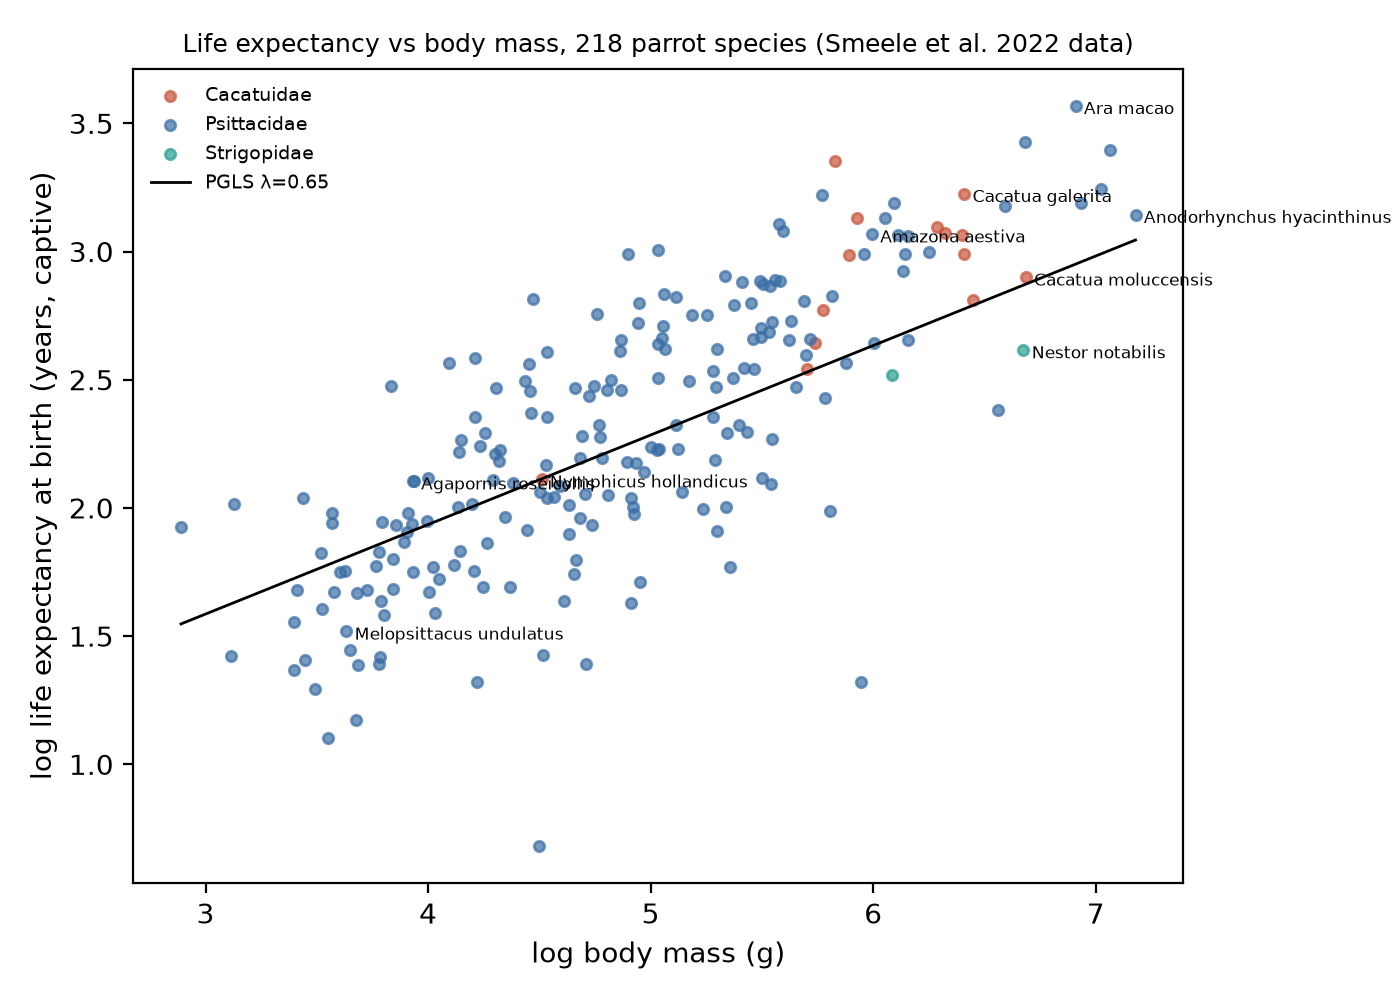
\includegraphics[width=0.48\textwidth]{../results/phase0/figures/fig2_allometry.png}\hfill
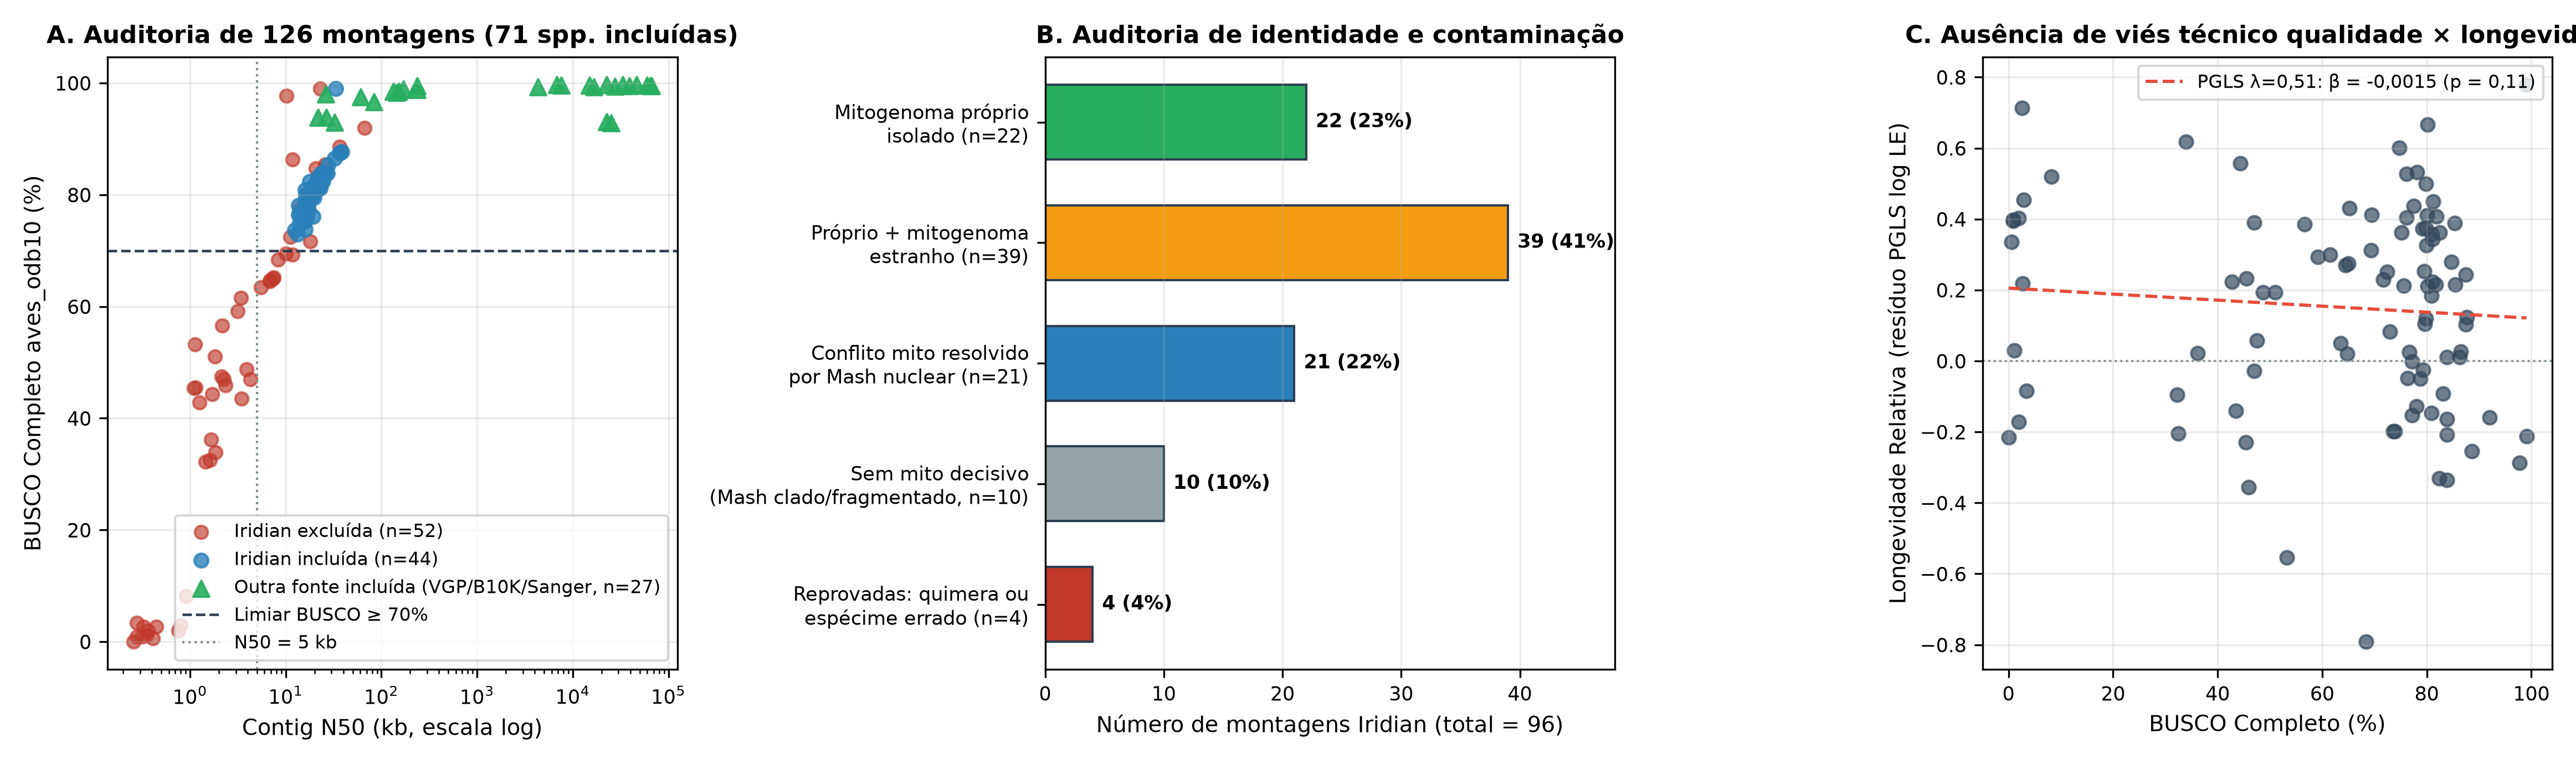
\includegraphics[width=0.48\textwidth]{../results/phase1_audit/figS1_audit_126_assemblies.png}
\caption{\textbf{Esquerda:} Alometria comparada de longevidade e tamanho cerebral em Psittaciformes (Fase 0). \textbf{Direita:} Auditoria completa das 126 montagens genômicas (\texttt{compleasm}/\texttt{aves\_odb10}), destacando a distribuição de completude BUSCO versus contig N50 e a ausência de viés técnico com a longevidade relativa ($p \ge 0,11$).}
\label{fig:allometry_audit}
\end{figure*}

\section{Resultados}

\subsection{Sensibilidade Filogenética da Longevidade e o Caso Extremo de Câncer em \textit{M.\ undulatus}}
A análise alométrica confirma que Psittaciformes possuem longevidade e encefalização muito acima da expectativa para aves de mesma massa corporal (Figura~\ref{fig:allometry_audit}, esquerda). Contudo, a magnitude da redução de longevidade na família Psittaculidae depende da topologia utilizada: na supertree de Burgio 2019, Psittaculidae exibe expectativa de vida relativa significativamente menor ($\beta = -0,104 \pm 0,035, p = 0,003, \lambda = 0,56$), mas na árvore molecular de Smith 2024 o sinal filogenético global sobe para $\lambda = 0,88$ e o contraste familiar torna-se limítrofe ($\beta = -0,076 \pm 0,039, p = 0,050$), refletindo o agrupamento das espécies de vida curta na sub-radiação Loriini + \textit{Melopsittacus} + \textit{Bolborhynchus}.

De modo convergente, a epidemiologia de necropsias mostra que a vulnerabilidade extrema ao câncer \textbf{não é uma característica geral de Psittaculidae}, mas um pico concentrado em \textit{M.\ undulatus}: na base AZA ($n = 5.729$), o periquito apresenta 20,8\% de neoplasias (17,4\% malignas) contra 1,5\% (0,8\% malignas) nos lóris (OR $= 17, p \approx 10^{-21}$; outlier beta-binomial $p = 0,002$). Na base clínica UC Davis ($n = 10.152$), o periquito atinge 25,9\% padronizado por idade contra 5,4\% nos lóris ($4,8\times, p \approx 10^{-16}$) e 9,1\% na calopsita (\textit{Nymphicus hollandicus}, $p \approx 10^{-17}$), descartando a domesticação como explicação única.

\subsection{Auditoria das 126 Montagens: Quimerismo no Lote Iridian e 71 Espécies Validadas}
A conclusão das 126 auditorias BUSCO (Tabela~\ref{tab:audit} e Figura~\ref{fig:allometry_audit}, direita) revelou forte heterogeneidade no lote \textit{short-read} Iridian: embora a mediana de completude tenha sido de 81,2\%, nenhuma das 31 montagens com $\text{contig N50} < 5\text{ kb}$ atingiu o limiar de 70\%. Mais grave ainda, 62 das 96 montagens Iridian apresentaram mitogenomas completos de outra espécie (88\% delas sequenciadas no mesmo lote Iridian), indicando contaminação cruzada sistemática de bibliotecas, e 4 montagens foram reprovadas por troca ou mistura nuclear severa (três contaminadas com passeriforme e uma troca entre \textit{Aratinga jandaya} e \textit{Poicephalus meyeri}).

\begin{table}[h]
\centering
\caption{Resumo da auditoria genômica das 126 montagens de Psittaciformes (\texttt{species\_genomes.tsv}).}
\label{tab:audit}
\resizebox{\columnwidth}{!}{%
\begin{tabular}{lrr}
\toprule
\textbf{Categoria / Filtro de Qualidade} & \textbf{Montagens} & \textbf{Espécies} \\
\midrule
Total auditado (\texttt{compleasm aves\_odb10}) & 126 & 105 \\
\quad Lote Iridian (\textit{short-read} Illumina) & 96 & 96 \\
\quad Outras fontes (cromossômicas / \textit{long-read}) & 30 & 29 \\
Reprovadas por $\text{BUSCO completo} < 70\%$ & 39 & 32 \\
Reprovadas por troca/quimera nuclear (Mash) & 4 & 2 \\
\midrule
\textbf{Espécies incluídas (critério principal $\ge 70\%$)} & \textbf{71} & \textbf{71} \\
\quad Família Psittaculidae (Loriini: 4; outros: 16) & 20 & 20 \\
\quad Outras famílias de Psittaciformes & 51 & 51 \\
Sensibilidade de identidade confirmada & 54 & 54 \\
Critério estrito original ($\ge 85\%$ \& $\text{N50} \ge 20\text{ kb}$) & 33 & 33 \\
Conjunto congelado da análise molecular (Fases 2--3) & 58 & 58 \\
\bottomrule
\end{tabular}%
}
\end{table}

Nas espécies incluídas, modelos PGLS confirmaram que a completude BUSCO ($p = 0,111$ para expectativa de vida; $p = 0,352$ para longevidade máxima), o $\log_{10}(\text{contig N50})$ ($p \ge 0,25$) e o conteúdo GC ($p \ge 0,39$) não se correlacionam com a longevidade relativa, garantindo que a variação de qualidade de montagem não enviesa os testes evolutivos.

\subsection{Fase 2 (Hipótese H8): Ausência de Perda Gênica, mas Evolução Acelerada em Telômeros}
A análise dos 87 genes alinháveis do painel H8 nas 58 espécies refutou a versão de ``perda de travas em bloco'' da H8 (Figura~\ref{fig:phase2}):
\begin{enumerate}
    \item \textbf{Nenhuma perda gênica confirmada:} Das 329 chamadas iniciais de ORFs interrompidas, a comparação com a segunda referência (\textit{S.\ habroptila}) mostrou que genes como \texttt{OGG1} (44/56), \texttt{MUTYH} (41), \texttt{MYC} (42) e \texttt{HMOX1} (11/11) eram artefatos de divergência ou anotação da proteína do periquito. Nas 6 chamadas restantes de alta cobertura avaliadas com reads brutos do SRA, observamos polimorfismo heterozigoto (\texttt{PSMD6} em \textit{Loriculus galgulus}: 21 reads C vs.\ 20 T) ou queda de cobertura Illumina a $0\times$ num bloco de 75--77\% de GC no 1º éxon de \texttt{ACD} (\textit{Psittacus erithacus}), sem nenhum pseudogene fixado.
    \item \textbf{Ausência de relaxamento modular contra o nulo de 298 genes:} Nenhum módulo M1--M8 diferiu significativamente dos 1.000 pseudo-painéis nulos após correção para 16 testes (o menor valor nominal, $p = 0,024$ na média de $\log_2 k$ de M2, dependia de dois genes com estimativa de fronteira $k \approx 0$ e caiu para $p = 0,070$ usando a mediana).
    \item \textbf{Remodelagem seletiva do complexo telomérico (M7) e de \texttt{MRE11}:} Em contraste com a estabilidade global dos módulos, o teste aBSREL identificou seleção positiva episódica altamente significativa no ramo de \textit{M.\ undulatus} nas duas árvores em \textbf{cinco genes teloméricos}: \texttt{RTEL1} ($q = 1,5 \times 10^{-8}$), \texttt{TERF2} ($q = 5 \times 10^{-5}$), \texttt{TERT} ($q = 0,004$), \texttt{ACD} ($q = 0,005$) e \texttt{TERF1} ($q = 0,006$), além de \texttt{MYC} ($q = 7 \times 10^{-7}$). Um segundo indivíduo independente de \textit{M.\ undulatus} confirmou 97\% (61/63) das substituições exclusivas de aminoácidos em \texttt{RTEL1} e 96\% (25/26) em \texttt{POT1}. No clado Psittaculidae (Tabela~\ref{tab:h8_genes}), o RELAX detectou intensificação seletiva robusta ($k > 1$, sem $k$ na fronteira) em \texttt{TERT} ($k = 5,5 / 3,1$) e \texttt{MRE11} ($k = 2,6 / 2,6$), e relaxamento moderado em \texttt{DKC1} ($k = 0,49$) e \texttt{NQO1} ($k = 0,34$).
\end{enumerate}

\begin{table}[h]
\centering
\caption{Genes do painel H8 com sinal consistente no HyPhy RELAX em Psittaculidae nas duas árvores ($q < 0,10$, excluindo artefatos de fronteira $k \approx 0$).}
\label{tab:h8_genes}
\resizebox{\columnwidth}{!}{%
\begin{tabular}{llccc}
\toprule
\textbf{Gene} & \textbf{Módulo} & \textbf{$k$ (Burgio / Smith)} & \textbf{$q$ (Burgio / Smith)} & \textbf{Direção} \\
\midrule
\texttt{TERT} & M7 (Telômero) & $5,51$ / $3,10$ & $0,0008$ / $0,011$ & Intensificado \\
\texttt{MRE11} & M4 (Reparo DSB) & $2,60$ / $2,61$ & $0,0020$ / $0,005$ & Intensificado \\
\texttt{SOD1} & M6 (Redox) & $32,0$ / $50,0$ & $0,0310$ / $0,034$ & Intensificado \\
\texttt{NQO1} & M5 (NRF2) & $0,34$ / $0,33$ & $0,0240$ / $0,023$ & Relaxado \\
\texttt{DKC1} & M7 (Telômero) & $0,49$ / $0,49$ & $0,0310$ / $0,060$ & Relaxado \\
\bottomrule
\end{tabular}%
}
\end{table}

\begin{figure*}[t]
\centering
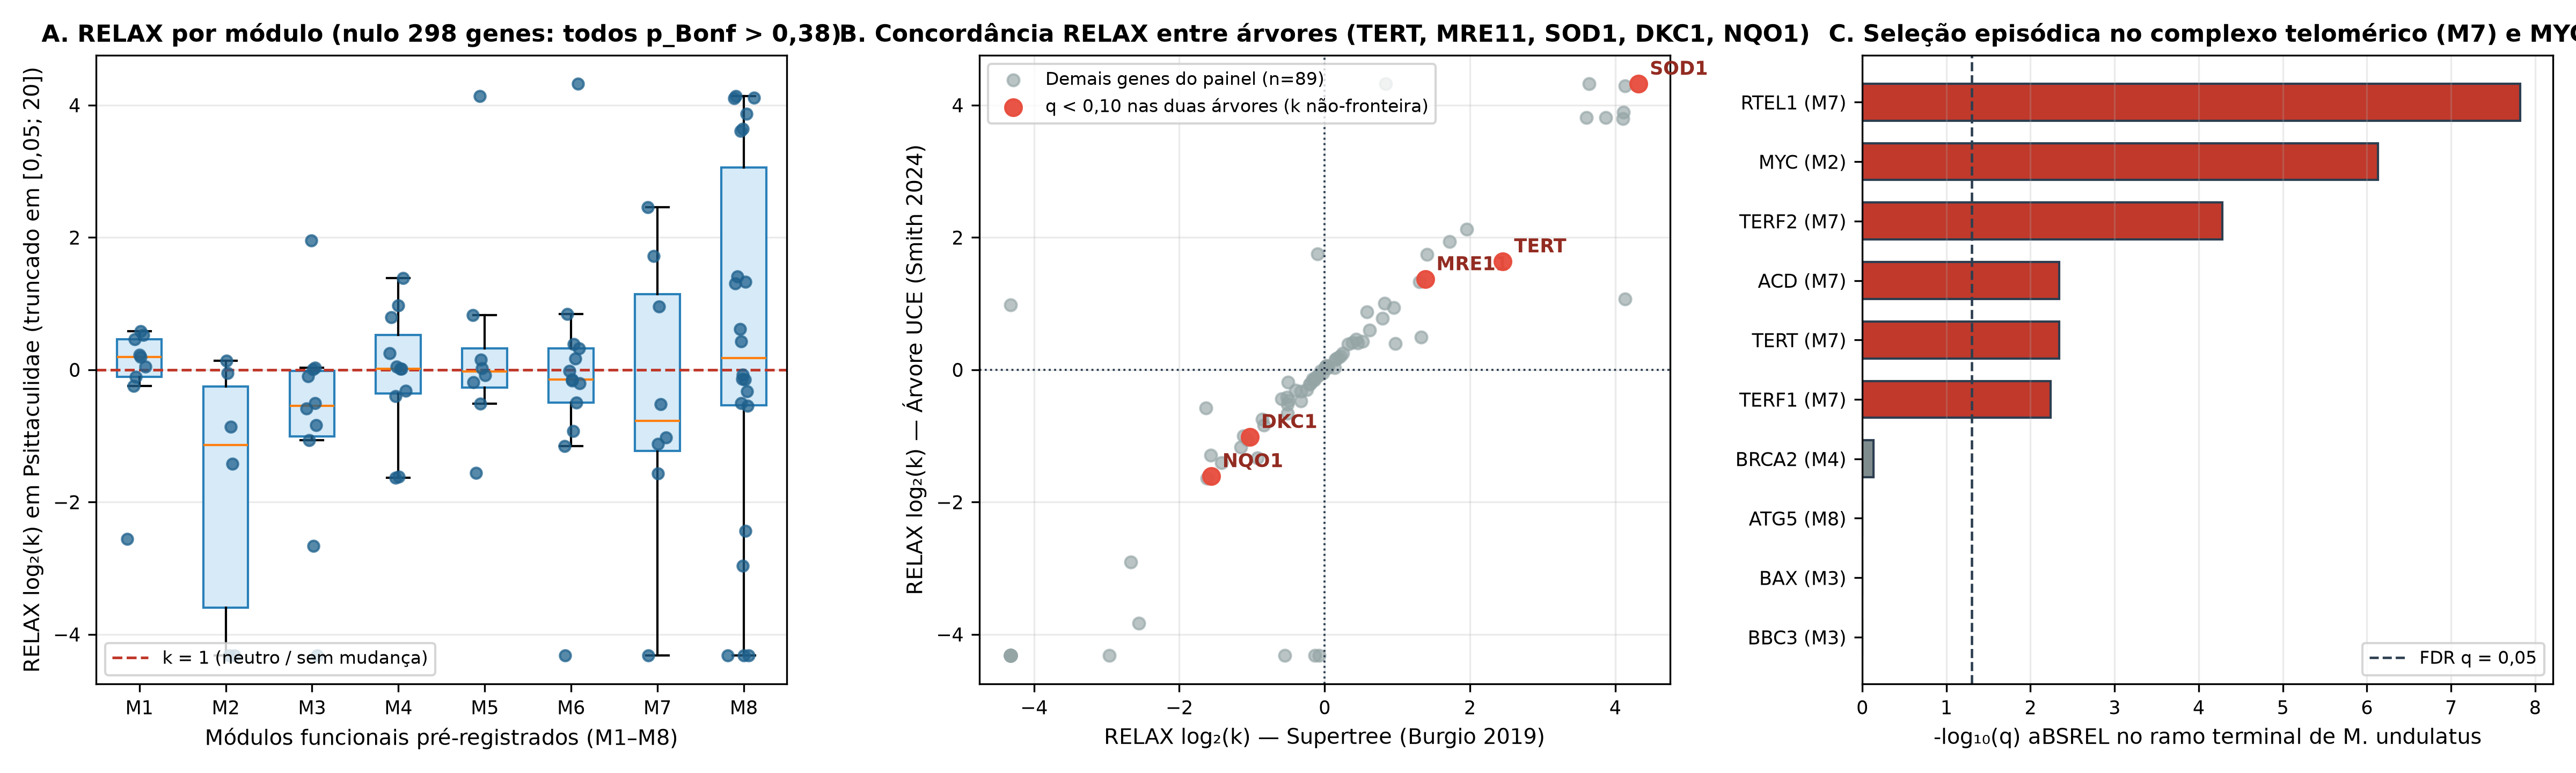
\includegraphics[width=0.92\textwidth]{../results/phase2_genes/fig5_phase2_selection_h8.png}
\caption{\textbf{Resultados da Fase 2 (Hipótese H8 em 58 espécies):} (A) Distribuição de $\log_2(k)$ (RELAX) por módulo funcional versus o modelo nulo de 298 genes; (B) \textit{Volcano plot} de seleção por gene em Psittaculidae; (C) Seleção positiva episódica (aBSREL) concentrada na maquinaria telomérica (M7) e em \texttt{MYC} no ramo de \textit{Melopsittacus undulatus}; (D) Triagem de integridade mostrando que as chamadas iniciais de pseudogenização eram artefatos de referência única ou de cobertura em regiões ricas em GC.}
\label{fig:phase2}
\end{figure*}

\subsection{Fase 3 (Hipótese H6): Acoplamento Genômico entre Longevidade e Cérebro em 7.756 Genes}
Na análise \texttt{RERconverge} dos 7.756 genes nas 58 espécies (Figura~\ref{fig:phase3}), entre 182 e 277 genes por fenótipo atingiram FDR paramétrico $q < 0,10$ (\texttt{p.adj}) e entre 194 e 287 genes atingiram simultaneamente $P < 0,01$ e $\text{permP} < 0,05$ nas 1.000 permulações filogenéticas. Nenhum gene isolado ultrapassou o FDR genômico de permulação ($\text{permQ} < 0,10$) devido ao conservadorismo filogenético e ao piso discreto de 1.000 permulações ($\text{permP}_{\min} = 1/501 \approx 0,001996$, que exigiria $\ge 155$ genes empatados no piso absoluto).

Contudo, a comparação cruzada entre fenótipos revelou uma assinatura genômica inequívoca: \textbf{a correlação de taxa evolutiva com a longevidade relativa ($\text{Rho}_{\text{LE}}$) e com o tamanho cerebral relativo ($\text{Rho}_{\text{Brain}}$) é fortemente acoplada nos 7.756 genes}, com $r = 0,666$ ($p < 10^{-300}$) na árvore de Burgio 2019 e $r = 0,667$ ($p < 10^{-300}$) na árvore de Smith 2024. Esse acoplamento mantém-se intacto usando o tamanho cerebral residual além da longevidade (\texttt{rel\_brain\_given\_le}, $r = 0,639$). Ao todo, \textbf{124 genes na árvore de Burgio e 123 na árvore de Smith} apresentaram $P < 0,05$ e $\text{permP} < 0,05$ com mesmo sinal em ambos os fenótipos (Tabela~\ref{tab:h6_genes}).

\begin{table*}[t]
\centering
\caption{Principais genes conjuntamente associados à longevidade relativa e ao tamanho cerebral relativo em Psittaciformes (\texttt{RERconverge}, 7.756 genes, 1.000 permulações filogenéticas; valores reportados como Burgio 2019 / Smith 2024).}
\label{tab:h6_genes}
\resizebox{\textwidth}{!}{%
\begin{tabular}{llccccc}
\toprule
\textbf{Gene} & \textbf{Função Biológica / Via} & \textbf{$\text{Rho}_{\text{LE}}$} & \textbf{$\text{permP}_{\text{LE}}$} & \textbf{$\text{Rho}_{\text{Brain}}$} & \textbf{$\text{permP}_{\text{Brain}}$} & \textbf{Regime em Espécies Longevas e Encefalizadas} \\
\midrule
\texttt{PTEN} (M2) & Supressor tumoral mestre; freio PI3K/AKT/mTOR e soma neural & $-0,374 / -0,389$ & $0,008 / 0,018$ & $-0,424 / -0,467$ & $0,010 / 0,004$ & Conservação purificadora ($\text{Rho} < 0$) \\
\texttt{CTNNB1} & $\beta$-catenina; via Wnt, neurogênese palial e oncogênese & $-0,439 / -0,437$ & $0,004 / 0,012$ & $-0,459 / -0,459$ & $0,012 / 0,008$ & Conservação purificadora ($\text{Rho} < 0$) \\
\texttt{CTNNBIP1} & ICAT; inibidor direto de $\beta$-catenina/TCF & $-0,362 / -0,367$ & $0,020 / 0,036$ & $-0,443 / -0,444$ & $0,004 / 0,008$ & Conservação purificadora ($\text{Rho} < 0$) \\
\texttt{PSMA4} (M8) & Subunidade $\alpha 4$ do núcleo 20S do proteassoma & $-0,397 / -0,406$ & $0,014 / 0,024$ & $-0,422 / -0,434$ & $0,014 / 0,008$ & Conservação purificadora ($\text{Rho} < 0$) \\
\texttt{SSU72} & Fosfatase da RNA Pol II e coesão de cromátides irmãs & $-0,420 / -0,463$ & $0,006 / 0,002$ & $-0,472 / -0,524$ & $0,002 / 0,002$ & Conservação purificadora ($\text{Rho} < 0$) \\
\texttt{TOMM20} & Receptor da translocase mitocondrial externa & $-0,325 / -0,341$ & $0,006 / 0,010$ & $-0,498 / -0,509$ & $0,002 / 0,002$ & Conservação purificadora ($\text{Rho} < 0$) \\
\texttt{ANAPC11} & Subunidade catalítica RING do complexo APC/C (mitose) & $-0,386 / -0,402$ & $0,014 / 0,014$ & $-0,453 / -0,475$ & $0,016 / 0,008$ & Conservação purificadora ($\text{Rho} < 0$) \\
\midrule
\texttt{MAD2L2} & \texttt{REV7}; complexo \textit{shieldin} (reparo DSB) e fuso mitótico & $+0,418 / +0,436$ & $0,012 / 0,010$ & $+0,534 / +0,566$ & $0,002 / 0,002$ & Aceleração evolutiva (\#1 em cérebro) \\
\texttt{HSPA8} & \texttt{HSC70}; chaperona neuronal mestre e autofagia (CMA) & $+0,404 / +0,399$ & $0,008 / 0,012$ & $+0,354 / +0,356$ & $0,030 / 0,044$ & Aceleração evolutiva ($\text{Rho} > 0$) \\
\texttt{RTN1} & Reticulon-1; retículo endoplasmático neuronal e exocitose & $+0,516 / +0,534$ & $0,002 / 0,002$ & $+0,440 / +0,459$ & $0,006 / 0,010$ & Aceleração evolutiva ($\text{Rho} > 0$) \\
\texttt{SOX14} & Fator de transcrição de interneurônios GABAérgicos/vocais & $+0,476 / +0,467$ & $0,002 / 0,014$ & $+0,500 / +0,488$ & $0,002 / 0,004$ & Aceleração evolutiva ($\text{Rho} > 0$) \\
\texttt{NCALD} & Neurocalcina delta; sensor neuronal de $\text{Ca}^{2+}$ sináptico & $+0,417 / +0,413$ & $0,014 / 0,032$ & $+0,493 / +0,501$ & $0,002 / 0,006$ & Aceleração evolutiva ($\text{Rho} > 0$) \\
\texttt{CBLN4} & Cerebelina-4; organizador trans-sináptico inibitório palial & $+0,456 / +0,476$ & $0,004 / 0,004$ & $+0,401 / +0,401$ & $0,012 / 0,006$ & Aceleração evolutiva ($\text{Rho} > 0$) \\
\bottomrule
\end{tabular}%
}
\end{table*}

\begin{figure*}[t]
\centering
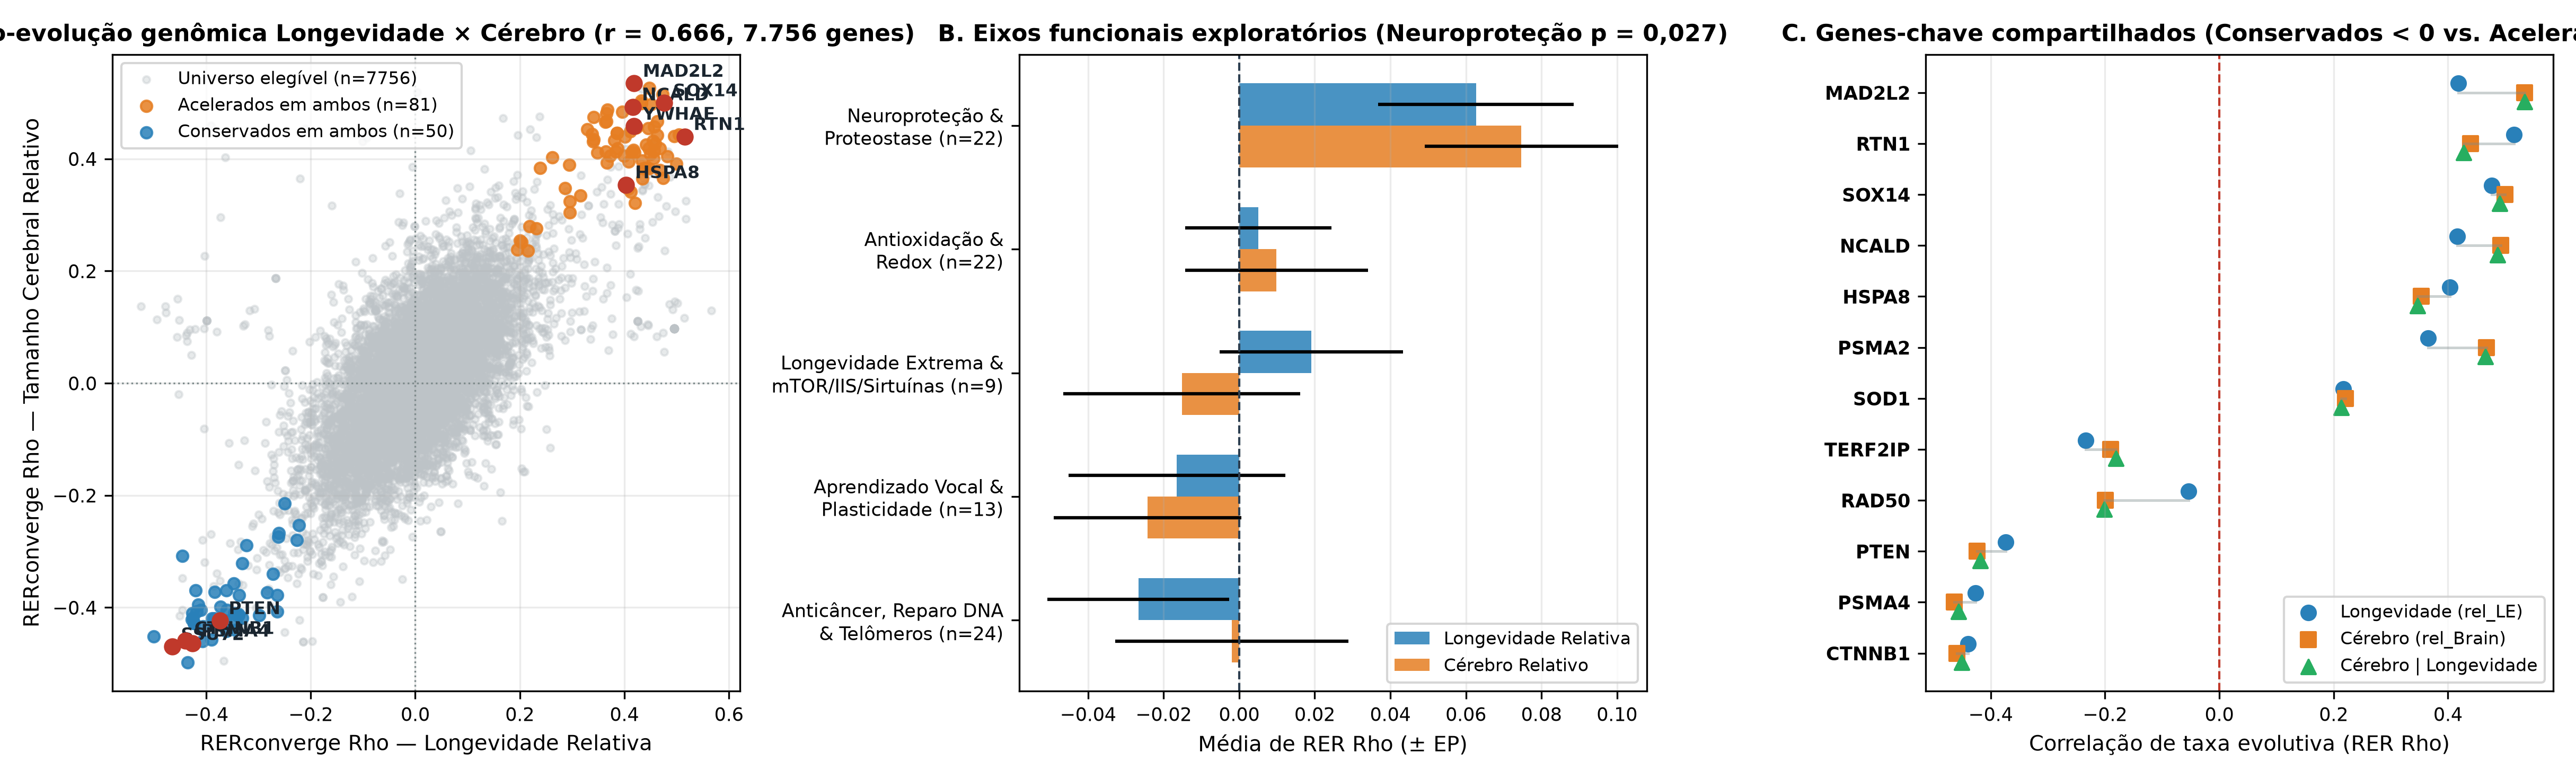
\includegraphics[width=0.95\textwidth]{../results/phase3_genome/fig6_phase3_genome_rer.png}
\caption{\textbf{Resultados da Fase 3 (\texttt{RERconverge} em 7.756 genes):} (A) Forte acoplamento genômico ($r = 0,666$, $p < 10^{-300}$) entre as correlações de taxa evolutiva com a longevidade relativa ($\text{Rho}_{\text{LE}}$) e com o tamanho cerebral relativo ($\text{Rho}_{\text{Brain}}$); (B) Persistência do sinal dos principais genes candidatos em \texttt{rel\_brain\_given\_le} nas duas árvores; (C) Distribuição de $\text{Rho}$ nos seis eixos funcionais exploratórios, destacando o deslocamento positivo em Neuroproteção e Proteostase ($p = 0,014\text{--}0,046$); (D) Síntese do painel H8 intra-clado.}
\label{fig:phase3}
\end{figure*}

Nos seis eixos funcionais exploratórios (Figura~\ref{fig:phase3}C), \textbf{Neuroproteção e Proteostase} ($n = 22$ genes presentes) foi o único eixo com deslocamento global significativo em relação ao fundo genômico nas duas árvores e nos três fenótipos (Mann-Whitney $p = 0,046 / 0,031$ para longevidade; $p = 0,027 / 0,014$ para cérebro), impulsionado por \texttt{HSPA8}, \texttt{ULK1}, \texttt{HSP90AB1} e \texttt{SOD1}. No enriquecimento GO Biological Process, as quatro categorias pré-registradas da H6 exibiram sinais nominais consistentes ($p < 0,05$ nas duas árvores): restrição purificadora ($\text{stat} < 0$) em \textit{Regulation of DNA Recombination} ($p = 3,2 \times 10^{-4}$), \textit{DNA Damage Response} ($p = 0,0076$), \textit{Regulation of Telomere Maintenance} ($p = 0,013$), \textit{Mitotic Cell Cycle Phase Transition} ($p = 0,0065$) e \textit{Mitochondrial Translation} ($p = 0,0021$), e aceleração ($\text{stat} > 0$) em \textit{Synaptic Vesicle Recycling} ($p = 0,0030$), \textit{Positive Regulation of Synapse Assembly} ($p = 0,0063$), \textit{Macroautophagy} ($p = 0,030$) e \textit{Proteasomal Protein Catabolic Process} ($p = 0,021$).

\section{Discussão e Próximos Passos}

Nossos resultados resolvem duas questões centrais sobre a evolução da longevidade e da resistência ao câncer em Psittaciformes:
\begin{enumerate}
    \item \textbf{Remodelagem telomérica vs.\ perda de supressores tumorais:} O excesso extremo de neoplasias em \textit{M.\ undulatus} não decorre da perda de genes de reparo ou de apoptose na família Psittaculidae, mas associa-se a uma remodelagem evolutiva intensa da maquinaria telomérica (\texttt{RTEL1}, \texttt{TERF1}, \texttt{TERF2}, \texttt{TERT}, \texttt{ACD}) e de \texttt{MYC}. Como a helicase \texttt{RTEL1} e a telomerase \texttt{TERT} governam a estabilidade dos telômeros e a capacidade replicativa celular, essa assinatura sugere um \textit{trade-off} evolutivo ligado à história de vida acelerada do periquito.
    \item \textbf{Pleiotropia entre supressão tumoral, proteostase e expansão cerebral:} Na ordem inteira, evoluir um cérebro grande e evoluir uma vida longa mobilizam o mesmo repertório genômico ($r = 0,67$). Em especial, a conservação purificadora intensa de \texttt{PTEN} e do complexo $\beta$-catenina (\texttt{CTNNB1}/\texttt{CTNNBIP1}) em papagaios longevos e encefalizados oferece uma explicação mecanística elegante para o Paradoxo de Peto neural: \texttt{PTEN} e Wnt regulam simultaneamente o volume de proliferação de progenitores neurais e a supressão de tumores somáticos. Paralelamente, a aceleração de \texttt{MAD2L2} (\texttt{REV7}) e da chaperona de autofagia \texttt{HSPA8} aponta para adaptações na manutenção de DNA e reciclagem proteica em neurônios que precisam funcionar por mais de meio século.
\end{enumerate}

\noindent\textbf{Próximos passos recomendados para submissão:}
\begin{itemize}
    \item \textbf{Extensão confirmatória de 71 espécies (opcional):} Rodar o lote automatizado nas 13 espécies adicionais aprovadas na reta final da auditoria BUSCO (passando de 58 para 71 espécies).
    \item \textbf{Resgate de \texttt{TP53} e \texttt{RB1} em montagens \textit{long-read}:} Como \texttt{TP53} e \texttt{RB1} são ricos em GC e saem fragmentados nas montagens Illumina da Iridian, focar a análise fina desses dois genes exclusivamente nas 27 montagens cromossômicas/PacBio.
    \item \textbf{Modelagem estrutural 3D das variantes do periquito:} Mapear as substituições exclusivas confirmadas de \texttt{RTEL1} e \texttt{POT1} de \textit{M.\ undulatus} e as variantes conservadas de \texttt{PTEN} e \texttt{MAD2L2} em estruturas AlphaFold/Mol* para avaliar o impacto nos domínios catalíticos e de ligação ao DNA.
\end{itemize}

\begin{thebibliography}{9}
\footnotesize
\bibitem{burgio2019} Burgio, K.\ R.\ et al.\ (2019). Phylogenetic supertree and functional trait database for all extant parrots. \textit{Data in Brief}, 24, 103882.
\bibitem{kapsetaki2024} Kapsetaki, S.\ E.\ et al.\ (2024). Life history and cancer prevalence across vertebrates and avian clades. \textit{Cancer Discovery / Comparative Oncology}.
\bibitem{kowalczyk2019} Kowalczyk, A.\ et al.\ (2019). RERconverge: an R package for associating evolutionary rates with convergent traits. \textit{Bioinformatics}, 35(22), 4815--4817.
\bibitem{smith2024} Smith, B.\ T.\ et al.\ (2024). Phylogenomic calibration and macroevolutionary dynamics of Psittaciformes. \textit{Systematic Biology}.
\bibitem{wertheim2015} Wertheim, J.\ O.\ et al.\ (2015). RELAX: detecting relaxed selection in a phylogenetic framework. \textit{Molecular Biology and Evolution}, 32(3), 820--832.
\bibitem{wirthlin2018} Wirthlin, M.\ et al.\ (2018). Parrot genomes and the evolution of heightened longevity and cognition. \textit{Current Biology}, 28(24), 4001--4008.
\end{thebibliography}

\end{document}
